\chapter{System Description}
\setlength{\parindent}{15pt}
\label{ch:syst_desc}

% what is this chapter about - Joel
In this chapter, the system will be considered on a deeper level of detail; the system is broken down into subsystems. In \autoref{sec:subs_inte} these subsystems are defined and the elements they are comprised of, are identified. \autoref{sec:inter} deals with the interrelations between the individual subsystems on design level; this is portrait by means of a N2 chart. \autoref{sec:subs_requ} states the subsystem requirements and constraints, which create the design space in which the design has to be performed. \autoref{sec:mass_cost_powe_brea} describe the mass, cost and power budget; the total budget is broken down and divided among the different subsystems. Since there is still an aspect of uncertainty at this stage of the design process, contingencies are incorporated in the budgets. These contingencies are justified in \autoref{sec:cont}.

\section{Subsystem Definition}
\label{sec:subs_inte}

%%% Subsystems introduction (5 sections) - Piotr
Subsystems are groups of elements within a system, which have a physical or functional commonality. Systems are divided into these groups in order to either have a better overview of the functionality or the design process, making it more approachable. The latter is especially valuable when working on larger projects such as the UAV system at hand, therefore it is sensible to split this system into subsystems as well. The subsystems and the responsible engineering departments are explained below, whilst the elements contained within each subsystem are listed in \autoref{tab:elem_subs}. \\

%explain structure of this section - relation, department allocation

%%% how we found subsystems - whiteboard image - Joel
\noindent \textbf{Structure: fuselage, wing, and tail:} Primarily, the main structural subsystems are addressed; the fuselage, the wing and the tail section. The fuselage is regarded as the main frame work; the attachments with the wing and the tail are regarded a 'fuselage' responsibility.

The first allocated department is the aerodynamics, due to the influence these subsystems have to the aerodynamic characteristics of the UAV.  Furthermore, the structures department is involved, because the fuselage, wing and tail form the main framework and thus the provide the structural integrity to the UAV.\\

\noindent \textbf{Propulsion:} Next to the main structural aspect, the propulsion is regarded as an individual subsystem; both physically and functionally. Physically it is developed and assembled separately, due to its external mounting. Furthermore, there are several top level requirement related to the VTOL capability and the high speed performance that are specific to the propulsion unit. Thus, functionally speaking, the propulsion system is regarded a separate subsystem as well.

The propulsion system includes the pylon, which forms the interface with the wing. This is regarded as a structural aspect. That is why the structural department is consulted in the development of the propulsion subsystem. Furthermore, there are several factors related to aerodynamics as well; not only the shape of the pylon, but also the feathered or folded propeller has strong affinity with the aerodynamics department. The propeller design itself is treated by the Power \& Propulsion department. Finally, the Control \& Stability will be involved, since stability and control is significantly related to the propulsion system, especially in vertical take of and hovering.\\

\noindent \textbf{Power:} The power management and distribution on board of the UAV is also selected to be its own subsystem. The main reason is that the only power source for all the other subsystems is electrical, making the power subsystem an essential and significant element of system. Due to its great importance, it requires a dedicated development section.

The Power \& Propulsion is the only department that will be involved in the design of the Power subsystem.\\

\noindent \textbf{Avionics and ground station:} Aviation related electronics that enable autonomous and supervised control lead up to the avionics and ground station subsystems. These two systems are composed of enough elements to be individual subsystems. \\ \indent The responsible department will be the Command \& Data Handling, since this department specialises in the data collection and processing within the UAS.\\

\noindent \textbf{Payload bay:} Although the payload bay was considered part of the fuselage section at first, later it was given a subsystem status. The subsystem needs to have a broad operational flexibility; there are several mission related requirement that result in a more complicated design. The resulting increased effort required for the design is so substantial, that it justifies the choice of making the payload bay a separate subsystem.\\ \indent Logically, the structures department is one of the involved parties; both for the implementation in the fuselage and for the payload hatches which enable drop-off mission. Besides structures, Command \& Data Handling will be involved to design the interface between the payload and the communication system. Also the interface with the power subsystem has to be considered; in some mission settings, the payload bay will be used to extent the battery capacity. That is why there is a connection with the Power \& Propulsion department.

\begin{table}[h]
\centering
\caption{Elements incorporated within subsystems}
\label{tab:elem_subs}
\begin{tabular}{lll}
\toprule
\textbf{Subsystems}     & \multicolumn{2}{c}{\textbf{Elements}}                               \\\midrule
\textbf{Fuselage}       & Internal layout            & Attachment fuselage - wing   \\
\textbf{}               & Structure                  & Attachment fuselage - tail   \\
\textbf{}               & Payload bay integration    & Battery mounting              \\\hdashline
\textbf{Wing}           & Control surface            & Structure                     \\
\textbf{}               & Actuator                   & Landing gear                  \\
\textbf{}               & High lift device           & Attachment wing - propulsion unit \\
                        & Wingtip devices            &                               \\\hdashline
\textbf{Tail}           & Structure                  & Actuator                      \\
\textbf{}               & Control surface            &                               \\\hdashline
\textbf{Propulsion}     & Motor                      & Storing/feathering mode       \\
\textbf{}               & Propellers                 & Motor controller              \\
\textbf{}               & Tilting mechanism          & Pylon structure               \\\hdashline
\textbf{Power}          & Battery unit               & Electrical elements           \\
\textbf{}               & Cable hardness             &                               \\\hdashline
\textbf{Avionics}       & Flight Control Module                        & Communication system          \\
\textbf{}               & Sensors                    & Autopilot                     \\
\textbf{}               & Navigation system          & Safety system                 \\\hdashline
\textbf{Payload}        & Payload mounting           & Data transmission             \\
\textbf{}               & Payload hatch              & Power connector               \\\hdashline
\textbf{Ground station} & CPU                        & Controller (input device)            \\
\textbf{}               & Display (visual interface) & Casing                        \\
                        & Communication system       & Power supply                  \\
                        & Maintenance unit           & Antenna tracking system       \\\bottomrule
\end{tabular}
\end{table}

\section{Subsystem Interrelations}
\label{sec:inter}

%%%% Piotr
Although the definition of the subsystems gives a general overview of the design process, it is not sufficient to be useful during the design process itself. To solve this problem, it is necessary to define the relations between the subsystems in the form of an $N^{2}$ chart. This makes it possible to determine beforehand which subsystems are most critical (i.e. have most dependants) and allows to plan a strategy in order to prevent any setbacks. In addition, it also shows which subsystems are highly dependent on the others (thus sensitive to design delays). Both of these features of the $N^{2}$ chart hint at which subsystems should be developed first, and which subsystems will be subject to larger changes at later design stages. Finally, the $N^{2}$ chart informs all the departments working on each of the subsystems about what information they need to supply to the other subsystems, resulting in a smoother design process flow.

%%% explain the function and method
%%% explain the interrelations
%%% N2; as a tool to show the design interrelations

The relations between the different subsystems in the design process of the UAS at hand are shown in the $N^{2}$ chart found on the next page. This chart should be interpreted clockwise; the inputs to the blocks are shown horizontally, the outputs are shown vertically. In the diagonal, the subsystems are shown with a list of the corresponding responsible departments underneath.

% general way = structural relations consists mostly of cg position dimensions etc.

The fuselage is the main framework of the UAV, that is why this subsystem has a substantial number of inputs. First of all, there are the general inputs; these are subsystem masses and dimensions, as well as forces and moments introduces by these subsystem. These are needed for the structural aspect of the interfaces between the fuselage and the subsystems. For stability purposes also the masses, locations of component such as battery and sensors, and c.g. position of units such as the wing and tail are needed. Furthermore also the aerodynamic centres and lift values of the wing and tail are needed.  

The wing can be, for the most part, designed independently from the rest of the UAV. Although it greatly depends on the masses of the subsystems, the design is only influenced by the overall mass, not singular contributions. The wing design is also influenced by the fuselage and propulsion subsystems, yet to a much lesser extent since these subsystems only define the design of the connection points on the wing. Therefore those areas will require design inputs such as the wing configuration (high, mid, or low wing), or the  engine mount (pylon) geometry. In addition, the forces and moments introduced by the propulsion will have to be known.

The inputs to the tail subsystem mostly consists of the aerodynamic interference related parameters of the wing and the propeller with the tail (wash). Since the tail has to provide stability and controllability, some control \& stability related parameters are input to the tail design as well.

The propulsion is most critical to the VTOL stability and controllability, therefore this subsystem requires inputs related to the disposition of the engine mounts on the wing, and the overall c.g. of the aircraft.

The power subsystem needs to provide sufficient power to overcome drag and (in the case of VTOL) the weight. That is why there is a relation between the drag generated by different subsystems and the power system. For the weight input, the overall mass is used (similarly to the mass input for the wing). Furthermore, the power consumption of the avionics and payload is influencing the power system and therefore it is also part of the inputs.

The payload bay requires outputs from the fuselage such that it is possible to integrate it inside the fuselage structure. In addition, several mission require the payload to send data to the ground station. Therefore this subsystem needs outputs from the avionics subsystem ensuring a compatible communication, and outputs from the power subsystem in order to be able to power the payload equipment.

Finally, the ground station is only directly related to the avionics subsystem. The input from the avionics are the signal related parameters, such as the signal strength. This is also the other way around; avionics is also just linked directly to the ground station, meaning that the inputs to the avionics will also be signal related parameters.


%%alter n2 chart 1) weight=mass, 2) remove masses 3) indicate in text the budget input into the prop and wing subsystem

%The first three blocks consists of the structures related subsystem, that is why much interrelation can be observed.



\newpage

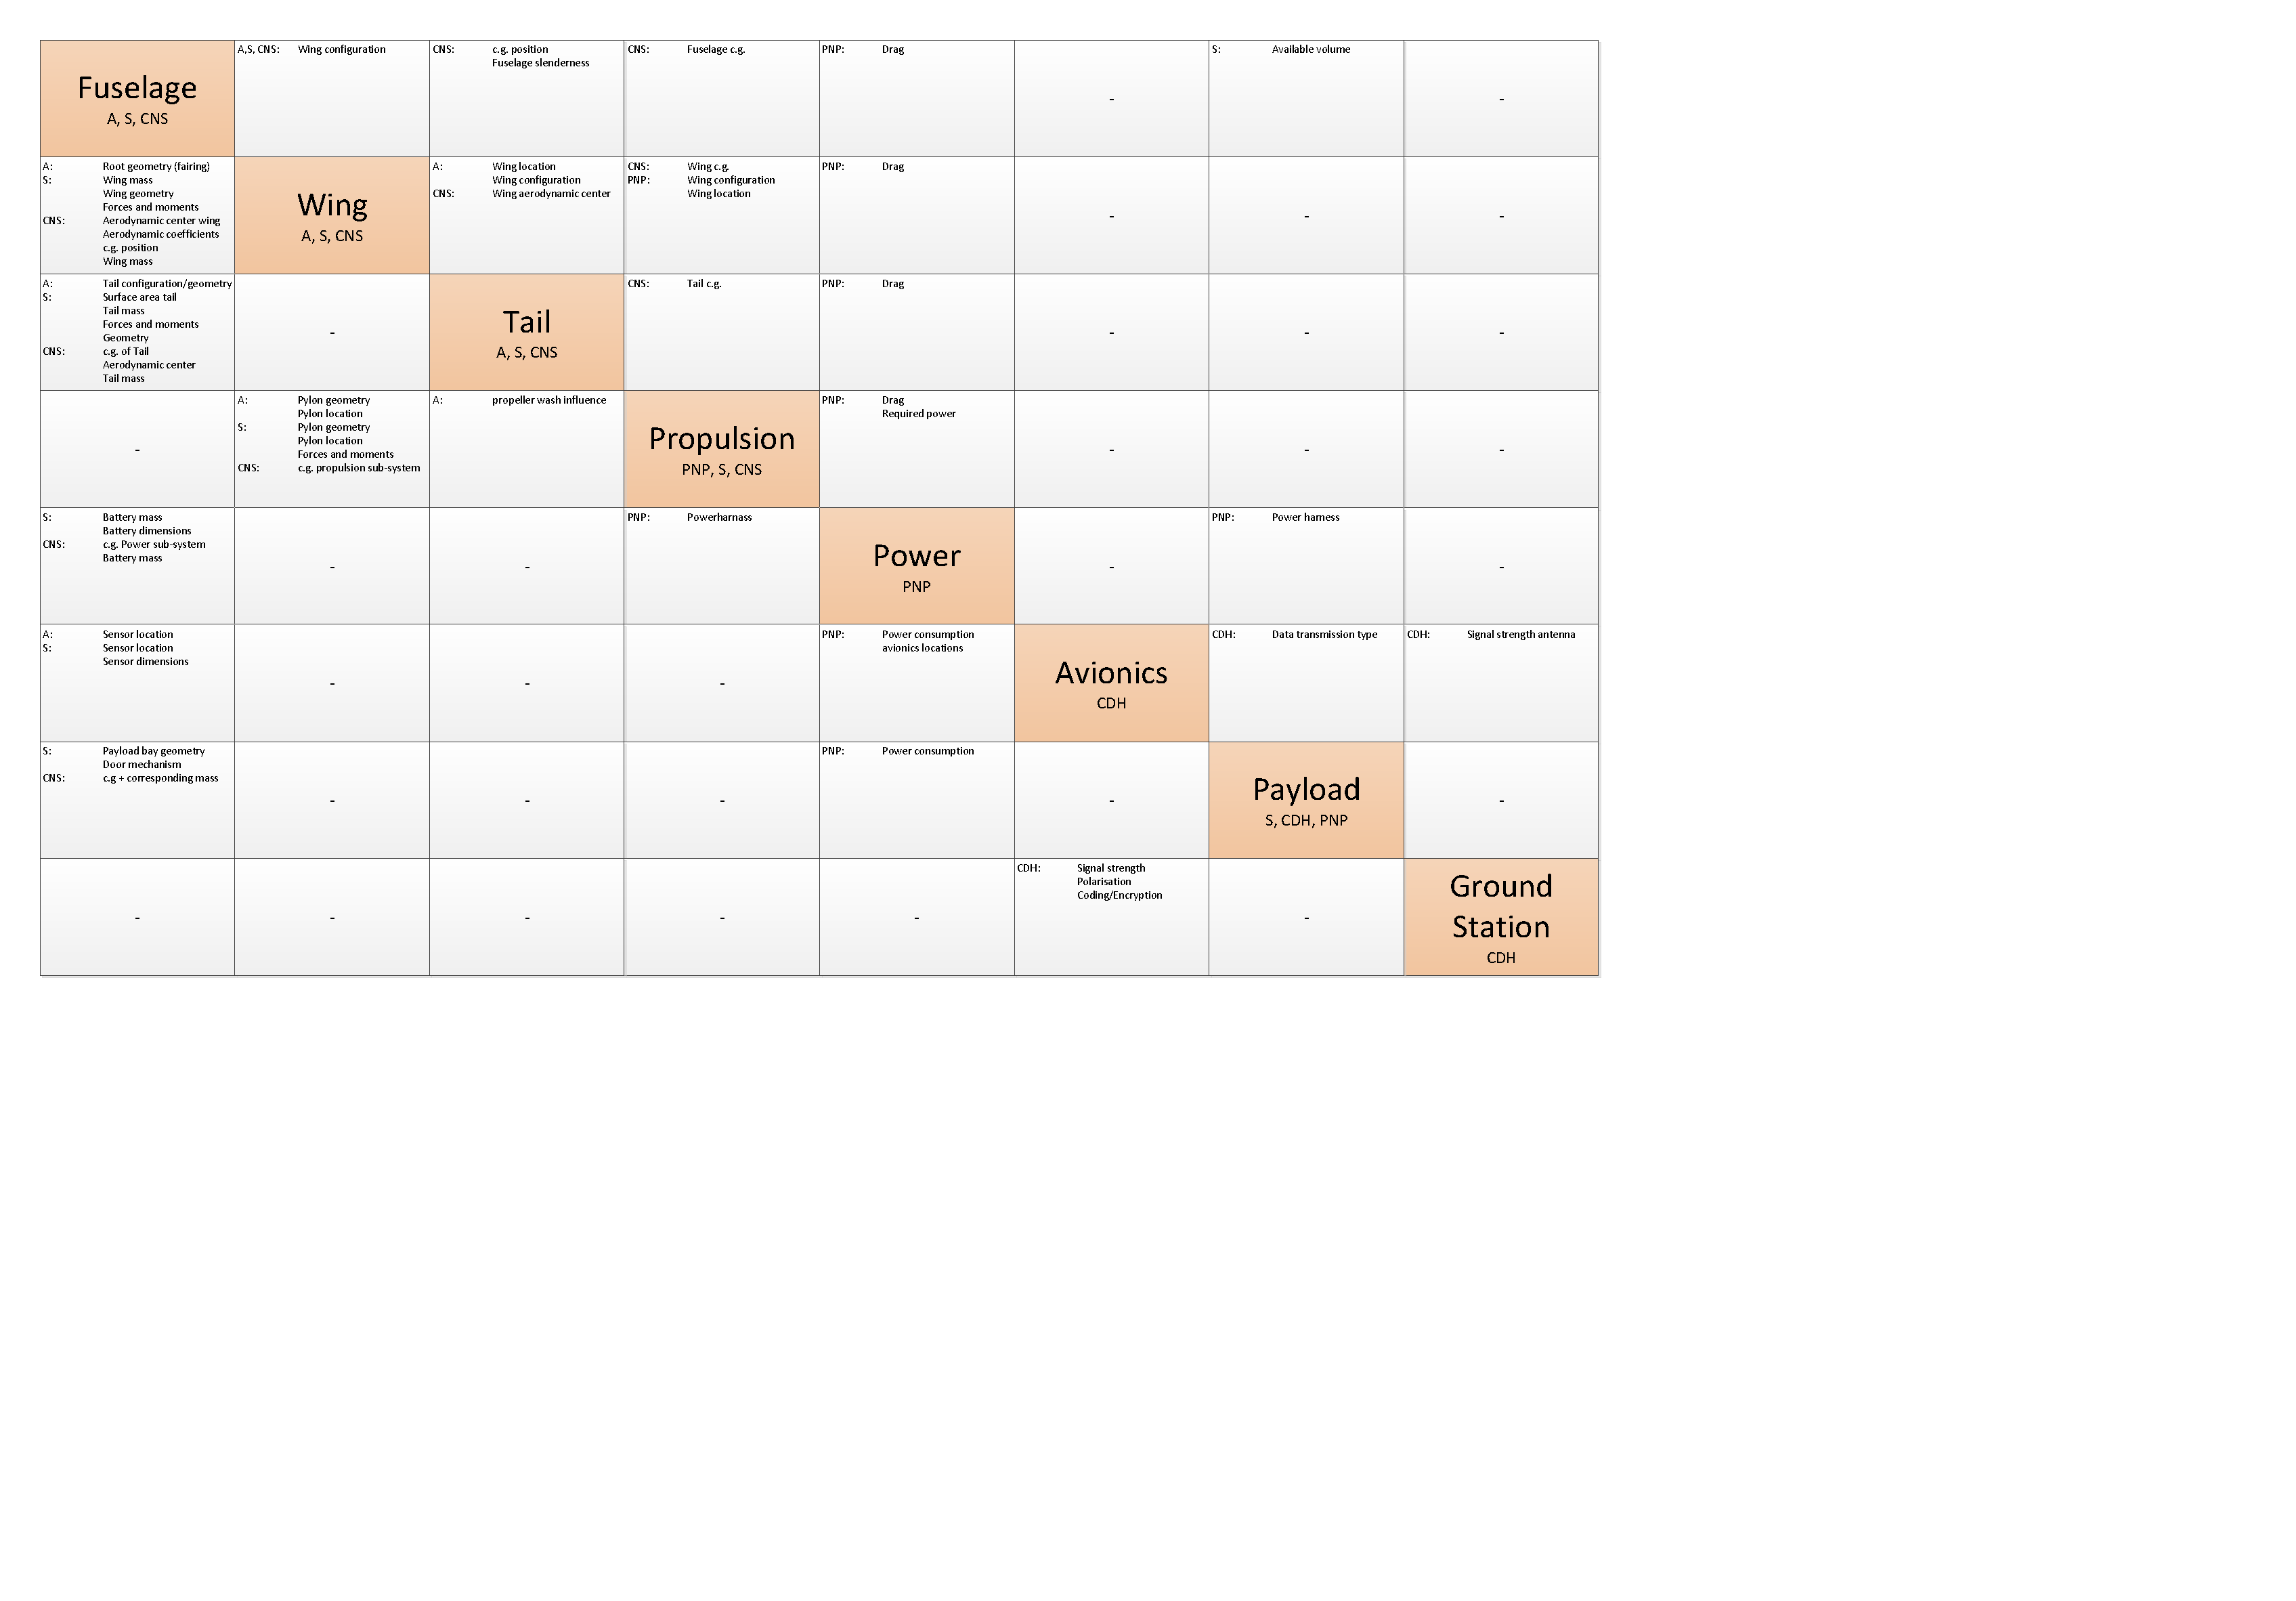
\includepdf[pages=1,fitpaper, scale=0.85,pagecommand={}]{SystemDescription/Figures/N2.pdf}
\label{N2}

\section{Subsystem Requirements}
\label{sec:subs_requ}

\section{Mass, Cost \& Power Breakdown}
\label{sec:mass_cost_powe_brea}

\section{Budget \& Contingencies}
\label{sec:cont}

